In this chapter, we introduce the first step of our hierarchical localization method: a \ac{cbir} method tuned for localization (see section~\ref{subsec:vbl_as_image_retrieval}). More precisely, we are interested in the design of a efficient global image descriptor for long-term localization.

As discussed in the previous chapter, one of the main challenges of \ac{vbl} remains the mapping of images acquired under changing conditions: cross-season images matching~\cite{Naseer2017a}, comparison of recent images with reference data collected a long time ago~\cite{Toft2018}, day to night place recognition~\cite{Torii2015}, etc. Recent approaches use complementary information in order to address these visually challenging localization scenarios: geometric information through point cloud~\cite{Sattler2018,Schonberger2017a} or depth maps~\cite{Christie2016} and semantic information~\cite{Ardeshir2014,Christie2016,Naseer2017a}. However geometric or semantic information are not always available or can be costly to obtain, especially in robotics or mobile applications when the sensor or the computational load on the system is limited, or in digital humanities when the data belong to ancient collections. 

In this work, we are considering a scenario where we have an offline access to multi-modal data but only-radiometric information during the online localization step (as illustrated in figure~\ref{fig:data_setup}). This is a realistic scenario: a mobile mapping vehicle with multiple sensors is used once to gather initial information on the area of interest and then, agents are sending localization request with a low computational sensor like a smart-phone camera. Such setup is also in accordance with the specifications of the \ac{plat} project (see section~\ref{subsec:platinum}), where this works is part of.

Based on these observations, we propose an image descriptor capable of reproducing the underlying scene geometry from a monocular image, in order to deal with challenging outdoor large-scale image-based localization scenarios. We introduce dense geometric information as side training objective to make our new descriptor robust to visual changes that occur between images taken at different times. Once trained, our system can be used on monocular images only to construct an expressive descriptor for image retrieval. This kind of system design is also known as side information learning~\cite{Hoffman2016}, as it uses geometric and radiometric information only during the training step and pure radiometric data for the image localization.  

The chapter is organized as follows. In section~\ref{sec:cbir_data_for_loc}, we first revisit recent works related to image description for localization and side information learning approaches. In section~\ref{sec:preliminary_work}, we describe our first approach to build a strong image descriptor trained with side depth information followed, in section~\ref{sec:method}, by the presentation of our final architecture. In section~\ref{sec:impl_details} we give insight on our implementation and on the dataset we used and we illustrate the effectiveness of the proposed method on six localization scenarios in section~\ref{sec:experiments}. We discuss, in section~\ref{sec:chall_loc}, about the challenging night to day image matching problem and, in section~\ref{sec:modality_ref}, we present a variation of our method using dense object reflectance map instead of depth maps. Section~\ref{sec:conclusion} finally concludes the chapter.

\begin{figure}
	\centering
		
	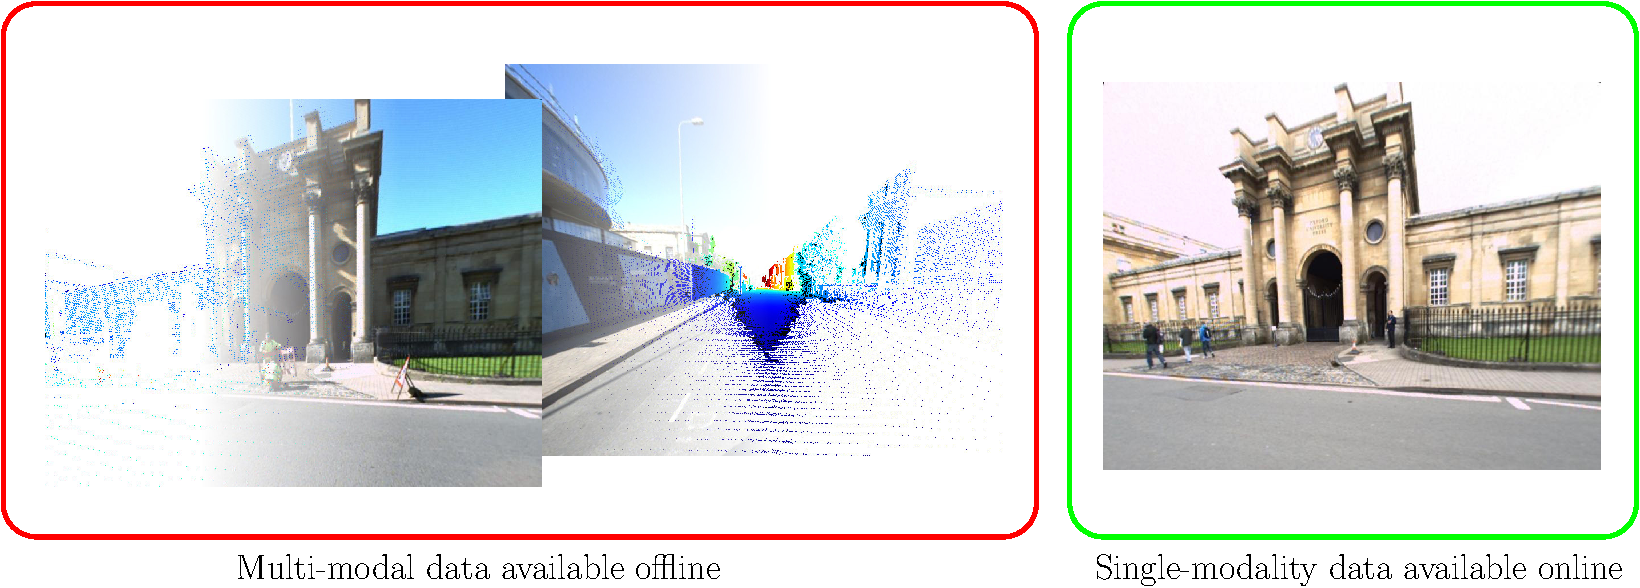
\includegraphics[width=\linewidth]{introduction/data_setup}

	\caption[Data partitioning]{\label{fig:data_setup} \textbf{Data partitioning within a practical localization scenario:} data available offline are richer than the one used during the localization task. We consider RGB (radiometric) + D (geometric) + R (material reflectance) as multi-modal data and only-RGB as single modality information.}
	
\end{figure}
	